\documentclass[a4paper,12pt]{article}
\usepackage{graphicx}
\usepackage{amsmath}

\begin{document}

\title{Exercise Sheet 1}
\author{May 16, 2026}
\date{\today}
\maketitle

\section{Exercise 1}
We call a transition system $TS = (S, Act, \to, S_0, AP, L)$
\begin{itemize}
    \item action-deterministic if $\left|S_0\right| \leq 1$ and $\left|Post(s, \alpha)\right| \leq 1$ for all $s \in S$ and $\alpha \in Act$, and
    \item AP-deterministic if $\left|S_0\right| \leq 1$ and $\left|Post(s) \cap \{s' \in S \mid L(s') = A \} \right| \leq 1$ for all $s \in S$ and $A \in 2^{AP}$,
\end{itemize}
where $Post(s, \alpha) = \{s' \in S \mid \exists \left(s, \alpha, s'\right) \in \to\}$ and \\$Post(s) = \cup_{\alpha \in Act}Post(s,\alpha)$

Let the transition system $TS_1$ be as follows.

\begin{figure}[htbp]
    \centering
    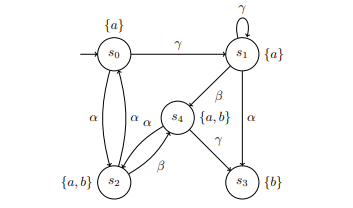
\includegraphics[width=0.7\textwidth]{mc-exercise-1.png}
\end{figure}

(a) Give the formal definition of $TS_1$

(b) Specify a finite and an infinite execution of $TS_1$

(c) Decide whether $TS_1$ is (i) AP-deterministic, and/or (ii) action-deterministic. Justify your answer.

\begin{center}
    \bfseries Solution
\end{center}

(a) The formal definition of $TS_1$:
\begin{itemize}
    \item State Space: $S = \{s_0, s_1, s_2, s_3, s_4\}$
    \item Action: $Act = \{\alpha, \beta, \gamma\}$
    \item Transition relation: 
    \begin{center}
        $\to = \{(s_0, \gamma, s_1),$ $(s_0, \alpha, s_2),$ $(s_1, \gamma, s_1),$ $(s_1, \beta, s_4),$ $(s_1, \alpha, s_3),$
                $(s_2, \alpha, s_0),$ $(s_2, \beta, s_4),$ $(s_4, \alpha, s_2),$ $(s_4, \gamma, s_3)\}$
    \end{center}
    \item Initial State: $S_0 = {s_0}$
    \item Atomic Propositions: $AP = \{a, b\}$
    \item Labeling Function:
    \[
        L(s) = \begin{cases} 
            \{a\} & \text{if } s \in \{s_0, s_1\} \\
            \{a, b\} & \text{if } s \in \{s_2, s_4\} \\
            \{b\} & \text{if } s = s_3 
        \end{cases}
    \]
\end{itemize}

(b) A finite execution of $TS_1$:
    \begin{center}
        $s_0 \xrightarrow{\alpha} s_2 \xrightarrow{\beta} s_4 \xrightarrow{\gamma} s_3$
    \end{center}

An infinite execution of $TS_1$:
    \begin{center}
        $(s_0 \xrightarrow{\alpha} s_2 \xrightarrow{\alpha} s_0) ^ \omega$
    \end{center}

(c) Based on what has been given, we have:
\begin{itemize}
    \item $\forall s \in S, \forall \alpha \in Act, \text{if } (\left|S_0\right| \leq 1) \land (\left|Post(s, \alpha)\right| \leq 1)$ $\implies$ Action-deterministic (1)
    \item $\forall s \in S, A \in 2^{AP}, \text{if } (\left|S_0\right| \leq 1) \land (\left|Post(s) \cap \{s' \in S \mid L(s') = A\}\right| \leq 1)$ $\implies$ AP-deterministic (2)
\end{itemize}

Because $\left|S_0\right| = 1 \implies \left|S_0\right| \leq 1 = True$ (3)

\begin{itemize}
    \item Check $TS_1$ is AP-deterministic
    
    $2^{AP}$ is the set of all subsets of AP
    $$2^{AP} = \{\phi, \{a\}, \{b\}, \{a, b\}\}$$

    From (2), (3) $\implies$ 
    
    For $TS_1$ is AP-deterministic, $\left|Post(s) \cap \{s' \in S \mid L(s') = A\}\right| \leq 1$ must be True
    \begin{itemize}
        \item With $s = s_0$:

            $Post(s_0) = \{s_1, s_2\}$

            \begin{itemize}
                \item[-] With $A = \phi$
                
                $\{s' \in S \mid L(s') = A\}$ = $\{\}$

                $\implies$  $\left|Post(s) \cap \{s' \in S \mid L(s') = A\}\right|$ $= \left|\{\}\right|$ $= 0 \leq 1$ (satisfied)
                \item[-] With $A = \{a\}$
                
                $\{s' \in S \mid L(s') = A\}$ = $\{s_0, s_1\}$

                $\implies$ $\left|Post(s) \cap \{s' \in S \mid L(s') = A\}\right|$ $= \left|\{s_1\}\right|$ $= 1 \leq 1$ (satisfied)
                \item[-] With $A = \{b\}$
            
                 $\{s' \in S \mid L(s') = A\}$ = $\{s_3\}$

                 $\implies$ $\left|Post(s) \cap \{s' \in S \mid L(s') = A\}\right|$ $= \left|\{\}\right|$ $= 0 \leq 1$ (satisfied)
                \item[-] With $A = \{a, b\}$ 
                
                 $\{s' \in S \mid L(s') = A\}$ = $\{s_2, s_4\}$

                 $\implies$ $\left|Post(s) \cap \{s' \in S \mid L(s') = A\}\right|$ $= \left|\{s_2\}\right|$ $= 1 \leq 1$ (satisfied)
            \end{itemize} 
        \item With $s = s_1$
           
            $Post(s_1) = \{s_3, s_4\}$

            \begin{itemize}
                \item[-] With $A = \phi$
                
                $\{s' \in S \mid L(s') = A\}$ = $\{\}$

                $\implies$  $\left|Post(s) \cap \{s' \in S \mid L(s') = A\}\right|$ $= \left|\{\}\right|$ $= 0 \leq 1$ (satisfied)
                \item[-] With $A = \{a\}$
                
                $\{s' \in S \mid L(s') = A\}$ = $\{s_0, s_1\}$

                $\implies$ $\left|Post(s) \cap \{s' \in S \mid L(s') = A\}\right|$ $= \left|\{\}\right|$ $= 0 \leq 1$ (satisfied)
                \item[-] With $A = \{b\}$
            
                 $\{s' \in S \mid L(s') = A\}$ = $\{s_3\}$

                 $\implies$ $\left|Post(s) \cap \{s' \in S \mid L(s') = A\}\right|$ $= \left|\{s_3\}\right|$ $= 1 \leq 1$ (satisfied)
                \item[-] With $A = \{a, b\}$ 
                
                 $\{s' \in S \mid L(s') = A\}$ = $\{s_2, s_4\}$

                 $\implies$ $\left|Post(s) \cap \{s' \in S \mid L(s') = A\}\right|$ $= \left|\{s_4\}\right|$ $= 1 \leq 1$ (satisfied)
            \end{itemize}
        \item With $s = s_2$
           
            $Post(s_2) = \{s_0, s_4\}$

            \begin{itemize}
                \item[-] With $A = \phi$
                
                $\{s' \in S \mid L(s') = A\}$ = $\{\}$

                $\implies$  $\left|Post(s) \cap \{s' \in S \mid L(s') = A\}\right|$ $= \left|\{\}\right|$ $= 0 \leq 1$ (satisfied)
                \item[-] With $A = \{a\}$
                
                $\{s' \in S \mid L(s') = A\}$ = $\{s_0, s_1\}$

                $\implies$ $\left|Post(s) \cap \{s' \in S \mid L(s') = A\}\right|$ $= \left|\{s_0\}\right|$ $= 1 \leq 1$ (satisfied)
                \item[-] With $A = \{b\}$
            
                 $\{s' \in S \mid L(s') = A\}$ = $\{s_3\}$

                 $\implies$ $\left|Post(s) \cap \{s' \in S \mid L(s') = A\}\right|$ $= \left|\{\}\right|$ $= 0 \leq 1$ (satisfied)
                \item[-] With $A = \{a, b\}$ 
                
                 $\{s' \in S \mid L(s') = A\}$ = $\{s_2, s_4\}$

                 $\implies$ $\left|Post(s) \cap \{s' \in S \mid L(s') = A\}\right|$ $= \left|\{s_4\}\right|$ $= 1 \leq 1$ (satisfied)
            \end{itemize}
        \item With $s = s_3$
        
            $Post(s_3) = \{\}$

            \begin{itemize}
                \item[-] With $A = \phi$
                
                $\{s' \in S \mid L(s') = A\}$ = $\{\}$

                $\implies$  $\left|Post(s) \cap \{s' \in S \mid L(s') = A\}\right|$ $= \left|\{\}\right|$ $= 0 \leq 1$ (satisfied)
                \item[-] With $A = \{a\}$
                
                $\{s' \in S \mid L(s') = A\}$ = $\{s_0, s_1\}$

                $\implies$ $\left|Post(s) \cap \{s' \in S \mid L(s') = A\}\right|$ $= \left|\{\}\right|$ $= 0 \leq 1$ (satisfied)
                \item[-] With $A = \{b\}$
            
                 $\{s' \in S \mid L(s') = A\}$ = $\{s_3\}$

                 $\implies$ $\left|Post(s) \cap \{s' \in S \mid L(s') = A\}\right|$ $= \left|\{\}\right|$ $= 0 \leq 1$ (satisfied)
                \item[-] With $A = \{a, b\}$ 
                
                 $\{s' \in S \mid L(s') = A\}$ = $\{s_2, s_4\}$

                 $\implies$ $\left|Post(s) \cap \{s' \in S \mid L(s') = A\}\right|$ $= \left|\{\}\right|$ $= 0 \leq 1$ (satisfied)
            \end{itemize}
        \item With $s = s_4$
          
            $Post(s_4) = \{s_2, s_3\}$

            \begin{itemize}
                \item[-] With $A = \phi$
                
                $\{s' \in S \mid L(s') = A\}$ = $\{\}$

                $\implies$  $\left|Post(s) \cap \{s' \in S \mid L(s') = A\}\right|$ $= \left|\{\}\right|$ $= 0 \leq 1$ (satisfied)
                \item[-] With $A = \{a\}$
                
                $\{s' \in S \mid L(s') = A\}$ = $\{s_0, s_1\}$

                $\implies$ $\left|Post(s) \cap \{s' \in S \mid L(s') = A\}\right|$ $= \left|\{\}\right|$ $= 0 \leq 1$ (satisfied)
                \item[-] With $A = \{b\}$
            
                 $\{s' \in S \mid L(s') = A\}$ = $\{s_3\}$

                 $\implies$ $\left|Post(s) \cap \{s' \in S \mid L(s') = A\}\right|$ $= \left|\{s_3\}\right|$ $= 1 \leq 1$ (satisfied)
                \item[-] With $A = \{a, b\}$ 
                
                 $\{s' \in S \mid L(s') = A\}$ = $\{s_2, s_4\}$

                 $\implies$ $\left|Post(s) \cap \{s' \in S \mid L(s') = A\}\right|$ $= \left|\{s_2\}\right|$ $= 1 \leq 1$ (satisfied)
            \end{itemize}
    \end{itemize}
    $\implies$ $\left|Post(s) \cap \{s' \in S \mid L(s') = A\}\right|$ $\leq 1$ = True (4)

    From (3), (4) $\implies$ $TS_1$ is AP-deterministic

    \item Check $TS_1$ is Action-deterministic
        
    From (1) and (3) $\implies$ For $TS_1$ is action-deterministic, $\left|Post(s, \alpha)\right| \leq 1$ must be True

    \begin{itemize}
        \item Case $s = s_0$:
        
        $Post(s_0, \gamma) = \{s_1\}$, $Post(s_0, \alpha) = \{s_2\}$ (satisfied)
        \item Case $s = s_1$:
        
        $Post(s_1, \beta) = \{s_4\}$, $Post(s_1, \alpha) = \{s_3\}$ (satisfied)
        \item Case $s = s_2$:
        
        $Post(s_2, \beta) = \{s_4\}$, $Post(s_2, \alpha) = \{s_0\}$ (satisfied)
        \item Case $s = s_3$: (satisfied because there are no way to reach to any state)
        \item Case $s = s_4$:
        
        $Post(s_4, \alpha) = \{s_2\}$, $Post(s_4, \gamma) = \{s_3\}$ (satisfied) 
    \end{itemize}
    $\implies$ $\left|Post(s, \alpha)\right| \leq 1$ = True (5)
    
    From (3), (5) $\implies$ $TS_1$ is action-deterministic
\end{itemize}

\section{Exercise 2}
Consider the following sequential hardware circuit in C 
\end{document}